
        \documentclass[spanish, 11pt]{exam}

        %These tell TeX which packages to use.
        \usepackage{array,epsfig}
        \usepackage{amsmath, textcomp}
        \usepackage{amsfonts}
        \usepackage{amssymb}
        \usepackage{amsxtra}
        \usepackage{amsthm}
        \usepackage{mathrsfs}
        \usepackage{color}
        \usepackage{multicol, xparse}
        \usepackage{verbatim}


        \usepackage[utf8]{inputenc}
        \usepackage[spanish]{babel}
        \usepackage{eurosym}

        \usepackage{graphicx}
        \graphicspath{{../img/}}
        \usepackage{pgf}



        \printanswers
        \nopointsinmargin
        \pointformat{}

        %Pagination stuff.
        %\setlength{\topmargin}{-.3 in}
        %\setlength{\oddsidemargin}{0in}
        %\setlength{\evensidemargin}{0in}
        %\setlength{\textheight}{9.in}
        %\setlength{\textwidth}{6.5in}
        %\pagestyle{empty}

        \let\multicolmulticols\multicols
        \let\endmulticolmulticols\endmulticols
        \RenewDocumentEnvironment{multicols}{mO{}}
         {%
          \ifnum#1=1
            #2%
          \else % More than 1 column
            \multicolmulticols{#1}[#2]
          \fi
         }
         {%
          \ifnum#1=1
          \else % More than 1 column
            \endmulticolmulticols
          \fi
         }
        \renewcommand{\solutiontitle}{\noindent\textbf{Sol:}\enspace}

        \newcommand{\samedir}{\mathbin{\!/\mkern-5mu/\!}}

        \newcommand{\class}{1º Bachillerato}
        \newcommand{\examdate}{\today}

        \newcommand{\tipo}{A}


        \newcommand{\timelimit}{50 minutos}



        \pagestyle{head}
        \firstpageheader{
\includegraphics[width=0.2\columnwidth]{header_left}}{\textbf{Departamento de Matemáticas\linebreak \class}\linebreak \examnum}{
\includegraphics[width=0.1\columnwidth]{header_right}}
        \runningheader{\class}{\examnum}{Página \thepage\ of \numpages}
        \runningheadrule

        \newcommand{\examnum}{Autoevaluación de Estadística y Probabilidad}
        \begin{document}
        \begin{questions}
        \question au31e01 - Se realiza una encuesta a un grupo de 10 personas acerca del número de veces que acuden a la peluquería a lo largo de un año, obteniéndose los siguientes resultados: 3 5 5 2 3 4 5 8 4 4 
        \begin{multicols}{2}
        \begin{parts} \part[1] Realiza una tabla de frecuencias  \begin{solution}   \\\begin{tabular}{rrrrrrr}
\hline
   x\_i &   f\_i &   F\_i &   h\_i &   H\_i &   \%\_i &   \%A\_i \\
\hline
     2 &     1 &     1 &   0.1 &   0.1 &    10 &     10 \\
     3 &     2 &     3 &   0.2 &   0.3 &    20 &     30 \\
     4 &     3 &     6 &   0.3 &   0.6 &    30 &     60 \\
     5 &     3 &     9 &   0.3 &   0.9 &    30 &     90 \\
     8 &     1 &    10 &   0.1 &   1   &    10 &    100 \\
\hline
\end{tabular}   \end{solution} \part[1] Realiza un diagrama de barras  \begin{solution}   \\ \resizebox{0.8\textwidth}{!}{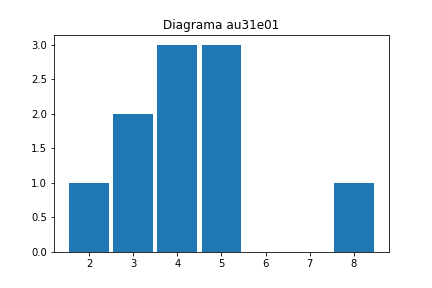
\includegraphics[width=1\columnwidth]{au31e01}}   \end{solution} \part[1] Calcular los parámetros de centralización  \begin{solution}   {'media': 4.3, 'mediana': 4.0, 'moda': ModeResult(mode=array([4]), count=array([3]))}   \end{solution} \part[1] Calcular los parámetros de posición P70, Q1, Q3, D4  \begin{solution}   {'P70': 5.0, 'Q1': 3.25, 'Q3': 5.0, 'D4': 4.0}   \end{solution} \part[1] Calcular los parámetros de dispersión  \begin{solution}   {'rango': 6, 'varianza': 2.41, 'desviación típica': 1.55241746962600, 'coeficiente variación': 0.361027318517675}   \end{solution}
        \end{parts}
        \end{multicols}
        \question au31e02 - En una consulta médica la distribución de pacientes por su edad ha sido, en la última semana, la siguiente:\\\begin{tabular}{rlr}
\hline
    & Duración               &   Cantidad \\
\hline
  0 & $\left[0, 30\right)$   &         10 \\
  1 & $\left[30, 60\right)$  &         20 \\
  2 & $\left[60, 90\right)$  &         25 \\
  3 & $\left[90, 120\right)$ &          3 \\
\hline
\end{tabular}
        \begin{multicols}{1}
        \begin{parts} \part[1] Haz una tabla de frecuencias  \begin{solution}   \begin{tabular}{rrrrrrrrrr}
\hline
    &   lim\_inf &   lim\_sup &   x\_i &   f\_i &   F\_i &       h\_i &        H\_i &   x\_if\_i &   x\^{}2\_if\_i \\
\hline
  0 &         0 &        30 &    15 &    10 &    10 & 0.172414  &   0.172414 &      150 &       2250 \\
  1 &        30 &        60 &    45 &    20 &    30 & 0.344828  &   0.517241 &      900 &      40500 \\
  2 &        60 &        90 &    75 &    25 &    55 & 0.431034  &   0.948276 &     1875 &     140625 \\
  3 &        90 &       120 &   105 &     3 &    58 & 0.0517241 &   1        &      315 &      33075 \\
  4 &       nan &       nan &   nan &    58 &   nan & 1         & nan        &     3240 &     216450 \\
\hline
\end{tabular}   \end{solution} \part[1] Calcula media, la varianza, la desviación típica y el coeficiente de variación  \begin{solution}   {'media': 55.86206896551724, 'varianza': 611.3258026159338, 'desviación típica': 24.7250035918285, 'coeficiente de variación': 0.442608088989523}   \end{solution} \part[1] La edad más frecuente de los pacientes  \begin{solution}   {'Intervalo modal': '$\\left[60.0, 90.0\\right)$', 'moda': 65.55555555555556}   \end{solution} \part[1] El percentil 47  \begin{solution}   {'k': 47, 'N': 58.0, '$L_i$': 30.0, '$f_i$': 20.0, '$F_{i-1}$': 10.0, '$C_i$': 30.0, 'percentil': 55.89}   \end{solution} \part[1] ¿Qué porcentaje de pacientes tenían una edad superior a 60 años?  \begin{solution}   {'valor': 60, 'N': 58.0, '$L_i$': 60.0, '$f_i$': 25.0, '$F_{i-1}$': 30.0, '$C_i$': 30.0, 'Porcentaje': 51.7241379310345}   \end{solution}
        \end{parts}
        \end{multicols}
        \question au31e03 - La temperatura media en los meses de invierno en varias ciudades y el gasto medio por habitante en
calefacción ha sido:\\\begin{tabular}{lrrrr}
\hline
                      &   0 &   1 &   2 &   3 \\
\hline
 Temperatura (grados) &  10 &  14 &  17 &  20 \\
 Gasto (euros)        & 150 & 102 &  55 &  18 \\
\hline
\end{tabular}
        \begin{multicols}{2}
        \begin{parts} \part[1] Haz una tabla de frecuencias con los datos que necesites para hace el resto de apartados  \begin{solution}   \begin{tabular}{rrrrrr}
\hline
    &   x &   y &   xy &   x2 &    y2 \\
\hline
  0 &  10 & 150 & 1500 &  100 & 22500 \\
  1 &  14 & 102 & 1428 &  196 & 10404 \\
  2 &  17 &  55 &  935 &  289 &  3025 \\
  3 &  20 &  18 &  360 &  400 &   324 \\
  4 &  61 & 325 & 4223 &  985 & 36253 \\
\hline
\end{tabular}   \end{solution} \part[1] Calcula el gasto medio  \begin{solution}   {'media': 81.25}   \end{solution} \part[1] Halla el coeficiente de correlación lineal e interprétalo  \begin{solution}   {'media de x': 15.25, 'desviación de x': 3.6996621467371855, 'media de y': 81.25, 'desviación de y': 49.61539579606314, 'covarianza': -183.3125, 'coeficiente de correlación': -0.9986505695692516}   \end{solution} \part[1] Estima el gasto medio por habitante de una ciudad si la temperatura media hubiera sido 12ºC  \begin{solution}   $y = - 13.3926940639269 x + 285.488584474886$ \\\resizebox {0.5\textwidth}{!}{%% Creator: Matplotlib, PGF backend
%%
%% To include the figure in your LaTeX document, write
%%   \input{<filename>.pgf}
%%
%% Make sure the required packages are loaded in your preamble
%%   \usepackage{pgf}
%%
%% Figures using additional raster images can only be included by \input if
%% they are in the same directory as the main LaTeX file. For loading figures
%% from other directories you can use the `import` package
%%   \usepackage{import}
%% and then include the figures with
%%   \import{<path to file>}{<filename>.pgf}
%%
%% Matplotlib used the following preamble
%%   \usepackage{fontspec}
%%   \setmainfont{DejaVuSerif.ttf}[Path=/home/hp/Mis_aplicaciones/anaconda3/lib/python3.6/site-packages/matplotlib/mpl-data/fonts/ttf/]
%%   \setsansfont{DejaVuSans.ttf}[Path=/home/hp/Mis_aplicaciones/anaconda3/lib/python3.6/site-packages/matplotlib/mpl-data/fonts/ttf/]
%%   \setmonofont{DejaVuSansMono.ttf}[Path=/home/hp/Mis_aplicaciones/anaconda3/lib/python3.6/site-packages/matplotlib/mpl-data/fonts/ttf/]
%%
\begingroup%
\makeatletter%
\begin{pgfpicture}%
\pgfpathrectangle{\pgfpointorigin}{\pgfqpoint{6.000000in}{4.000000in}}%
\pgfusepath{use as bounding box, clip}%
\begin{pgfscope}%
\pgfsetbuttcap%
\pgfsetmiterjoin%
\definecolor{currentfill}{rgb}{1.000000,1.000000,1.000000}%
\pgfsetfillcolor{currentfill}%
\pgfsetlinewidth{0.000000pt}%
\definecolor{currentstroke}{rgb}{1.000000,1.000000,1.000000}%
\pgfsetstrokecolor{currentstroke}%
\pgfsetdash{}{0pt}%
\pgfpathmoveto{\pgfqpoint{0.000000in}{0.000000in}}%
\pgfpathlineto{\pgfqpoint{6.000000in}{0.000000in}}%
\pgfpathlineto{\pgfqpoint{6.000000in}{4.000000in}}%
\pgfpathlineto{\pgfqpoint{0.000000in}{4.000000in}}%
\pgfpathclose%
\pgfusepath{fill}%
\end{pgfscope}%
\begin{pgfscope}%
\pgfsetbuttcap%
\pgfsetmiterjoin%
\definecolor{currentfill}{rgb}{1.000000,1.000000,1.000000}%
\pgfsetfillcolor{currentfill}%
\pgfsetlinewidth{0.000000pt}%
\definecolor{currentstroke}{rgb}{0.000000,0.000000,0.000000}%
\pgfsetstrokecolor{currentstroke}%
\pgfsetstrokeopacity{0.000000}%
\pgfsetdash{}{0pt}%
\pgfpathmoveto{\pgfqpoint{0.750000in}{0.500000in}}%
\pgfpathlineto{\pgfqpoint{5.400000in}{0.500000in}}%
\pgfpathlineto{\pgfqpoint{5.400000in}{3.520000in}}%
\pgfpathlineto{\pgfqpoint{0.750000in}{3.520000in}}%
\pgfpathclose%
\pgfusepath{fill}%
\end{pgfscope}%
\begin{pgfscope}%
\pgfpathrectangle{\pgfqpoint{0.750000in}{0.500000in}}{\pgfqpoint{4.650000in}{3.020000in}}%
\pgfusepath{clip}%
\pgfsetbuttcap%
\pgfsetroundjoin%
\definecolor{currentfill}{rgb}{0.121569,0.466667,0.705882}%
\pgfsetfillcolor{currentfill}%
\pgfsetfillopacity{0.800000}%
\pgfsetlinewidth{1.003750pt}%
\definecolor{currentstroke}{rgb}{0.121569,0.466667,0.705882}%
\pgfsetstrokecolor{currentstroke}%
\pgfsetstrokeopacity{0.800000}%
\pgfsetdash{}{0pt}%
\pgfpathmoveto{\pgfqpoint{0.967699in}{2.979571in}}%
\pgfpathcurveto{\pgfqpoint{0.978749in}{2.979571in}}{\pgfqpoint{0.989348in}{2.983962in}}{\pgfqpoint{0.997162in}{2.991775in}}%
\pgfpathcurveto{\pgfqpoint{1.004975in}{2.999589in}}{\pgfqpoint{1.009365in}{3.010188in}}{\pgfqpoint{1.009365in}{3.021238in}}%
\pgfpathcurveto{\pgfqpoint{1.009365in}{3.032288in}}{\pgfqpoint{1.004975in}{3.042887in}}{\pgfqpoint{0.997162in}{3.050701in}}%
\pgfpathcurveto{\pgfqpoint{0.989348in}{3.058515in}}{\pgfqpoint{0.978749in}{3.062905in}}{\pgfqpoint{0.967699in}{3.062905in}}%
\pgfpathcurveto{\pgfqpoint{0.956649in}{3.062905in}}{\pgfqpoint{0.946050in}{3.058515in}}{\pgfqpoint{0.938236in}{3.050701in}}%
\pgfpathcurveto{\pgfqpoint{0.930422in}{3.042887in}}{\pgfqpoint{0.926032in}{3.032288in}}{\pgfqpoint{0.926032in}{3.021238in}}%
\pgfpathcurveto{\pgfqpoint{0.926032in}{3.010188in}}{\pgfqpoint{0.930422in}{2.999589in}}{\pgfqpoint{0.938236in}{2.991775in}}%
\pgfpathcurveto{\pgfqpoint{0.946050in}{2.983962in}}{\pgfqpoint{0.956649in}{2.979571in}}{\pgfqpoint{0.967699in}{2.979571in}}%
\pgfpathclose%
\pgfusepath{stroke,fill}%
\end{pgfscope}%
\begin{pgfscope}%
\pgfpathrectangle{\pgfqpoint{0.750000in}{0.500000in}}{\pgfqpoint{4.650000in}{3.020000in}}%
\pgfusepath{clip}%
\pgfsetbuttcap%
\pgfsetroundjoin%
\definecolor{currentfill}{rgb}{0.121569,0.466667,0.705882}%
\pgfsetfillcolor{currentfill}%
\pgfsetfillopacity{0.800000}%
\pgfsetlinewidth{1.003750pt}%
\definecolor{currentstroke}{rgb}{0.121569,0.466667,0.705882}%
\pgfsetstrokecolor{currentstroke}%
\pgfsetstrokeopacity{0.800000}%
\pgfsetdash{}{0pt}%
\pgfpathmoveto{\pgfqpoint{2.653540in}{2.217172in}}%
\pgfpathcurveto{\pgfqpoint{2.664590in}{2.217172in}}{\pgfqpoint{2.675189in}{2.221562in}}{\pgfqpoint{2.683003in}{2.229376in}}%
\pgfpathcurveto{\pgfqpoint{2.690816in}{2.237190in}}{\pgfqpoint{2.695206in}{2.247789in}}{\pgfqpoint{2.695206in}{2.258839in}}%
\pgfpathcurveto{\pgfqpoint{2.695206in}{2.269889in}}{\pgfqpoint{2.690816in}{2.280488in}}{\pgfqpoint{2.683003in}{2.288301in}}%
\pgfpathcurveto{\pgfqpoint{2.675189in}{2.296115in}}{\pgfqpoint{2.664590in}{2.300505in}}{\pgfqpoint{2.653540in}{2.300505in}}%
\pgfpathcurveto{\pgfqpoint{2.642490in}{2.300505in}}{\pgfqpoint{2.631891in}{2.296115in}}{\pgfqpoint{2.624077in}{2.288301in}}%
\pgfpathcurveto{\pgfqpoint{2.616263in}{2.280488in}}{\pgfqpoint{2.611873in}{2.269889in}}{\pgfqpoint{2.611873in}{2.258839in}}%
\pgfpathcurveto{\pgfqpoint{2.611873in}{2.247789in}}{\pgfqpoint{2.616263in}{2.237190in}}{\pgfqpoint{2.624077in}{2.229376in}}%
\pgfpathcurveto{\pgfqpoint{2.631891in}{2.221562in}}{\pgfqpoint{2.642490in}{2.217172in}}{\pgfqpoint{2.653540in}{2.217172in}}%
\pgfpathclose%
\pgfusepath{stroke,fill}%
\end{pgfscope}%
\begin{pgfscope}%
\pgfpathrectangle{\pgfqpoint{0.750000in}{0.500000in}}{\pgfqpoint{4.650000in}{3.020000in}}%
\pgfusepath{clip}%
\pgfsetbuttcap%
\pgfsetroundjoin%
\definecolor{currentfill}{rgb}{0.121569,0.466667,0.705882}%
\pgfsetfillcolor{currentfill}%
\pgfsetfillopacity{0.800000}%
\pgfsetlinewidth{1.003750pt}%
\definecolor{currentstroke}{rgb}{0.121569,0.466667,0.705882}%
\pgfsetstrokecolor{currentstroke}%
\pgfsetstrokeopacity{0.800000}%
\pgfsetdash{}{0pt}%
\pgfpathmoveto{\pgfqpoint{3.917920in}{1.470656in}}%
\pgfpathcurveto{\pgfqpoint{3.928971in}{1.470656in}}{\pgfqpoint{3.939570in}{1.475046in}}{\pgfqpoint{3.947383in}{1.482860in}}%
\pgfpathcurveto{\pgfqpoint{3.955197in}{1.490673in}}{\pgfqpoint{3.959587in}{1.501272in}}{\pgfqpoint{3.959587in}{1.512323in}}%
\pgfpathcurveto{\pgfqpoint{3.959587in}{1.523373in}}{\pgfqpoint{3.955197in}{1.533972in}}{\pgfqpoint{3.947383in}{1.541785in}}%
\pgfpathcurveto{\pgfqpoint{3.939570in}{1.549599in}}{\pgfqpoint{3.928971in}{1.553989in}}{\pgfqpoint{3.917920in}{1.553989in}}%
\pgfpathcurveto{\pgfqpoint{3.906870in}{1.553989in}}{\pgfqpoint{3.896271in}{1.549599in}}{\pgfqpoint{3.888458in}{1.541785in}}%
\pgfpathcurveto{\pgfqpoint{3.880644in}{1.533972in}}{\pgfqpoint{3.876254in}{1.523373in}}{\pgfqpoint{3.876254in}{1.512323in}}%
\pgfpathcurveto{\pgfqpoint{3.876254in}{1.501272in}}{\pgfqpoint{3.880644in}{1.490673in}}{\pgfqpoint{3.888458in}{1.482860in}}%
\pgfpathcurveto{\pgfqpoint{3.896271in}{1.475046in}}{\pgfqpoint{3.906870in}{1.470656in}}{\pgfqpoint{3.917920in}{1.470656in}}%
\pgfpathclose%
\pgfusepath{stroke,fill}%
\end{pgfscope}%
\begin{pgfscope}%
\pgfpathrectangle{\pgfqpoint{0.750000in}{0.500000in}}{\pgfqpoint{4.650000in}{3.020000in}}%
\pgfusepath{clip}%
\pgfsetbuttcap%
\pgfsetroundjoin%
\definecolor{currentfill}{rgb}{0.121569,0.466667,0.705882}%
\pgfsetfillcolor{currentfill}%
\pgfsetfillopacity{0.800000}%
\pgfsetlinewidth{1.003750pt}%
\definecolor{currentstroke}{rgb}{0.121569,0.466667,0.705882}%
\pgfsetstrokecolor{currentstroke}%
\pgfsetstrokeopacity{0.800000}%
\pgfsetdash{}{0pt}%
\pgfpathmoveto{\pgfqpoint{5.182301in}{0.882973in}}%
\pgfpathcurveto{\pgfqpoint{5.193351in}{0.882973in}}{\pgfqpoint{5.203950in}{0.887363in}}{\pgfqpoint{5.211764in}{0.895177in}}%
\pgfpathcurveto{\pgfqpoint{5.219578in}{0.902991in}}{\pgfqpoint{5.223968in}{0.913590in}}{\pgfqpoint{5.223968in}{0.924640in}}%
\pgfpathcurveto{\pgfqpoint{5.223968in}{0.935690in}}{\pgfqpoint{5.219578in}{0.946289in}}{\pgfqpoint{5.211764in}{0.954102in}}%
\pgfpathcurveto{\pgfqpoint{5.203950in}{0.961916in}}{\pgfqpoint{5.193351in}{0.966306in}}{\pgfqpoint{5.182301in}{0.966306in}}%
\pgfpathcurveto{\pgfqpoint{5.171251in}{0.966306in}}{\pgfqpoint{5.160652in}{0.961916in}}{\pgfqpoint{5.152838in}{0.954102in}}%
\pgfpathcurveto{\pgfqpoint{5.145025in}{0.946289in}}{\pgfqpoint{5.140635in}{0.935690in}}{\pgfqpoint{5.140635in}{0.924640in}}%
\pgfpathcurveto{\pgfqpoint{5.140635in}{0.913590in}}{\pgfqpoint{5.145025in}{0.902991in}}{\pgfqpoint{5.152838in}{0.895177in}}%
\pgfpathcurveto{\pgfqpoint{5.160652in}{0.887363in}}{\pgfqpoint{5.171251in}{0.882973in}}{\pgfqpoint{5.182301in}{0.882973in}}%
\pgfpathclose%
\pgfusepath{stroke,fill}%
\end{pgfscope}%
\begin{pgfscope}%
\pgfpathrectangle{\pgfqpoint{0.750000in}{0.500000in}}{\pgfqpoint{4.650000in}{3.020000in}}%
\pgfusepath{clip}%
\pgfsetbuttcap%
\pgfsetroundjoin%
\definecolor{currentfill}{rgb}{0.121569,0.466667,0.705882}%
\pgfsetfillcolor{currentfill}%
\pgfsetfillopacity{0.150000}%
\pgfsetlinewidth{0.000000pt}%
\definecolor{currentstroke}{rgb}{0.000000,0.000000,0.000000}%
\pgfsetstrokecolor{currentstroke}%
\pgfsetdash{}{0pt}%
\pgfpathmoveto{\pgfqpoint{0.750000in}{3.382727in}}%
\pgfpathlineto{\pgfqpoint{0.750000in}{2.984769in}}%
\pgfpathlineto{\pgfqpoint{0.796970in}{2.962937in}}%
\pgfpathlineto{\pgfqpoint{0.843939in}{2.941106in}}%
\pgfpathlineto{\pgfqpoint{0.890909in}{2.919274in}}%
\pgfpathlineto{\pgfqpoint{0.937879in}{2.897443in}}%
\pgfpathlineto{\pgfqpoint{0.984848in}{2.875611in}}%
\pgfpathlineto{\pgfqpoint{1.031818in}{2.853780in}}%
\pgfpathlineto{\pgfqpoint{1.078788in}{2.831949in}}%
\pgfpathlineto{\pgfqpoint{1.125758in}{2.810117in}}%
\pgfpathlineto{\pgfqpoint{1.172727in}{2.788286in}}%
\pgfpathlineto{\pgfqpoint{1.219697in}{2.766454in}}%
\pgfpathlineto{\pgfqpoint{1.266667in}{2.744623in}}%
\pgfpathlineto{\pgfqpoint{1.313636in}{2.722791in}}%
\pgfpathlineto{\pgfqpoint{1.360606in}{2.700960in}}%
\pgfpathlineto{\pgfqpoint{1.407576in}{2.679128in}}%
\pgfpathlineto{\pgfqpoint{1.454545in}{2.657297in}}%
\pgfpathlineto{\pgfqpoint{1.501515in}{2.635465in}}%
\pgfpathlineto{\pgfqpoint{1.548485in}{2.613634in}}%
\pgfpathlineto{\pgfqpoint{1.595455in}{2.591802in}}%
\pgfpathlineto{\pgfqpoint{1.642424in}{2.569971in}}%
\pgfpathlineto{\pgfqpoint{1.689394in}{2.548139in}}%
\pgfpathlineto{\pgfqpoint{1.736364in}{2.526308in}}%
\pgfpathlineto{\pgfqpoint{1.783333in}{2.504477in}}%
\pgfpathlineto{\pgfqpoint{1.830303in}{2.482645in}}%
\pgfpathlineto{\pgfqpoint{1.877273in}{2.460814in}}%
\pgfpathlineto{\pgfqpoint{1.924242in}{2.438982in}}%
\pgfpathlineto{\pgfqpoint{1.971212in}{2.417151in}}%
\pgfpathlineto{\pgfqpoint{2.018182in}{2.395319in}}%
\pgfpathlineto{\pgfqpoint{2.065152in}{2.373488in}}%
\pgfpathlineto{\pgfqpoint{2.112121in}{2.351656in}}%
\pgfpathlineto{\pgfqpoint{2.159091in}{2.329825in}}%
\pgfpathlineto{\pgfqpoint{2.206061in}{2.307993in}}%
\pgfpathlineto{\pgfqpoint{2.253030in}{2.286162in}}%
\pgfpathlineto{\pgfqpoint{2.300000in}{2.264330in}}%
\pgfpathlineto{\pgfqpoint{2.346970in}{2.242499in}}%
\pgfpathlineto{\pgfqpoint{2.393939in}{2.220667in}}%
\pgfpathlineto{\pgfqpoint{2.440909in}{2.198836in}}%
\pgfpathlineto{\pgfqpoint{2.487879in}{2.177005in}}%
\pgfpathlineto{\pgfqpoint{2.534848in}{2.155173in}}%
\pgfpathlineto{\pgfqpoint{2.581818in}{2.133342in}}%
\pgfpathlineto{\pgfqpoint{2.628788in}{2.111510in}}%
\pgfpathlineto{\pgfqpoint{2.675758in}{2.089679in}}%
\pgfpathlineto{\pgfqpoint{2.722727in}{2.067847in}}%
\pgfpathlineto{\pgfqpoint{2.769697in}{2.046016in}}%
\pgfpathlineto{\pgfqpoint{2.816667in}{2.024184in}}%
\pgfpathlineto{\pgfqpoint{2.863636in}{2.002353in}}%
\pgfpathlineto{\pgfqpoint{2.910606in}{1.980521in}}%
\pgfpathlineto{\pgfqpoint{2.957576in}{1.958690in}}%
\pgfpathlineto{\pgfqpoint{3.004545in}{1.936858in}}%
\pgfpathlineto{\pgfqpoint{3.051515in}{1.915027in}}%
\pgfpathlineto{\pgfqpoint{3.098485in}{1.893195in}}%
\pgfpathlineto{\pgfqpoint{3.145455in}{1.871364in}}%
\pgfpathlineto{\pgfqpoint{3.192424in}{1.849533in}}%
\pgfpathlineto{\pgfqpoint{3.239394in}{1.827701in}}%
\pgfpathlineto{\pgfqpoint{3.286364in}{1.805870in}}%
\pgfpathlineto{\pgfqpoint{3.333333in}{1.784038in}}%
\pgfpathlineto{\pgfqpoint{3.380303in}{1.762207in}}%
\pgfpathlineto{\pgfqpoint{3.427273in}{1.740375in}}%
\pgfpathlineto{\pgfqpoint{3.474242in}{1.718544in}}%
\pgfpathlineto{\pgfqpoint{3.521212in}{1.696712in}}%
\pgfpathlineto{\pgfqpoint{3.568182in}{1.674881in}}%
\pgfpathlineto{\pgfqpoint{3.615152in}{1.653049in}}%
\pgfpathlineto{\pgfqpoint{3.662121in}{1.631218in}}%
\pgfpathlineto{\pgfqpoint{3.709091in}{1.609386in}}%
\pgfpathlineto{\pgfqpoint{3.756061in}{1.587555in}}%
\pgfpathlineto{\pgfqpoint{3.803030in}{1.565723in}}%
\pgfpathlineto{\pgfqpoint{3.850000in}{1.543892in}}%
\pgfpathlineto{\pgfqpoint{3.896970in}{1.522061in}}%
\pgfpathlineto{\pgfqpoint{3.943939in}{1.496961in}}%
\pgfpathlineto{\pgfqpoint{3.990909in}{1.469229in}}%
\pgfpathlineto{\pgfqpoint{4.037879in}{1.441497in}}%
\pgfpathlineto{\pgfqpoint{4.084848in}{1.413765in}}%
\pgfpathlineto{\pgfqpoint{4.131818in}{1.386033in}}%
\pgfpathlineto{\pgfqpoint{4.178788in}{1.358301in}}%
\pgfpathlineto{\pgfqpoint{4.225758in}{1.330569in}}%
\pgfpathlineto{\pgfqpoint{4.272727in}{1.302837in}}%
\pgfpathlineto{\pgfqpoint{4.319697in}{1.275106in}}%
\pgfpathlineto{\pgfqpoint{4.366667in}{1.247374in}}%
\pgfpathlineto{\pgfqpoint{4.413636in}{1.219642in}}%
\pgfpathlineto{\pgfqpoint{4.460606in}{1.191910in}}%
\pgfpathlineto{\pgfqpoint{4.507576in}{1.164178in}}%
\pgfpathlineto{\pgfqpoint{4.554545in}{1.136446in}}%
\pgfpathlineto{\pgfqpoint{4.601515in}{1.108714in}}%
\pgfpathlineto{\pgfqpoint{4.648485in}{1.080983in}}%
\pgfpathlineto{\pgfqpoint{4.695455in}{1.053251in}}%
\pgfpathlineto{\pgfqpoint{4.742424in}{1.025519in}}%
\pgfpathlineto{\pgfqpoint{4.789394in}{0.997787in}}%
\pgfpathlineto{\pgfqpoint{4.836364in}{0.970055in}}%
\pgfpathlineto{\pgfqpoint{4.883333in}{0.942323in}}%
\pgfpathlineto{\pgfqpoint{4.930303in}{0.914591in}}%
\pgfpathlineto{\pgfqpoint{4.977273in}{0.886860in}}%
\pgfpathlineto{\pgfqpoint{5.024242in}{0.859128in}}%
\pgfpathlineto{\pgfqpoint{5.071212in}{0.831396in}}%
\pgfpathlineto{\pgfqpoint{5.118182in}{0.803664in}}%
\pgfpathlineto{\pgfqpoint{5.165152in}{0.775932in}}%
\pgfpathlineto{\pgfqpoint{5.212121in}{0.748200in}}%
\pgfpathlineto{\pgfqpoint{5.259091in}{0.720468in}}%
\pgfpathlineto{\pgfqpoint{5.306061in}{0.692736in}}%
\pgfpathlineto{\pgfqpoint{5.353030in}{0.665005in}}%
\pgfpathlineto{\pgfqpoint{5.400000in}{0.637273in}}%
\pgfpathlineto{\pgfqpoint{5.400000in}{1.016788in}}%
\pgfpathlineto{\pgfqpoint{5.400000in}{1.016788in}}%
\pgfpathlineto{\pgfqpoint{5.353030in}{1.038030in}}%
\pgfpathlineto{\pgfqpoint{5.306061in}{1.059271in}}%
\pgfpathlineto{\pgfqpoint{5.259091in}{1.080512in}}%
\pgfpathlineto{\pgfqpoint{5.212121in}{1.101754in}}%
\pgfpathlineto{\pgfqpoint{5.165152in}{1.122995in}}%
\pgfpathlineto{\pgfqpoint{5.118182in}{1.144237in}}%
\pgfpathlineto{\pgfqpoint{5.071212in}{1.165478in}}%
\pgfpathlineto{\pgfqpoint{5.024242in}{1.186720in}}%
\pgfpathlineto{\pgfqpoint{4.977273in}{1.207961in}}%
\pgfpathlineto{\pgfqpoint{4.930303in}{1.229202in}}%
\pgfpathlineto{\pgfqpoint{4.883333in}{1.250444in}}%
\pgfpathlineto{\pgfqpoint{4.836364in}{1.271685in}}%
\pgfpathlineto{\pgfqpoint{4.789394in}{1.292927in}}%
\pgfpathlineto{\pgfqpoint{4.742424in}{1.314168in}}%
\pgfpathlineto{\pgfqpoint{4.695455in}{1.335410in}}%
\pgfpathlineto{\pgfqpoint{4.648485in}{1.356651in}}%
\pgfpathlineto{\pgfqpoint{4.601515in}{1.377892in}}%
\pgfpathlineto{\pgfqpoint{4.554545in}{1.399134in}}%
\pgfpathlineto{\pgfqpoint{4.507576in}{1.420375in}}%
\pgfpathlineto{\pgfqpoint{4.460606in}{1.441617in}}%
\pgfpathlineto{\pgfqpoint{4.413636in}{1.462858in}}%
\pgfpathlineto{\pgfqpoint{4.366667in}{1.484100in}}%
\pgfpathlineto{\pgfqpoint{4.319697in}{1.505341in}}%
\pgfpathlineto{\pgfqpoint{4.272727in}{1.526582in}}%
\pgfpathlineto{\pgfqpoint{4.225758in}{1.547824in}}%
\pgfpathlineto{\pgfqpoint{4.178788in}{1.569065in}}%
\pgfpathlineto{\pgfqpoint{4.131818in}{1.590307in}}%
\pgfpathlineto{\pgfqpoint{4.084848in}{1.611548in}}%
\pgfpathlineto{\pgfqpoint{4.037879in}{1.632790in}}%
\pgfpathlineto{\pgfqpoint{3.990909in}{1.654031in}}%
\pgfpathlineto{\pgfqpoint{3.943939in}{1.675272in}}%
\pgfpathlineto{\pgfqpoint{3.896970in}{1.696514in}}%
\pgfpathlineto{\pgfqpoint{3.850000in}{1.717755in}}%
\pgfpathlineto{\pgfqpoint{3.803030in}{1.738997in}}%
\pgfpathlineto{\pgfqpoint{3.756061in}{1.760238in}}%
\pgfpathlineto{\pgfqpoint{3.709091in}{1.781480in}}%
\pgfpathlineto{\pgfqpoint{3.662121in}{1.802721in}}%
\pgfpathlineto{\pgfqpoint{3.615152in}{1.823962in}}%
\pgfpathlineto{\pgfqpoint{3.568182in}{1.845204in}}%
\pgfpathlineto{\pgfqpoint{3.521212in}{1.866445in}}%
\pgfpathlineto{\pgfqpoint{3.474242in}{1.887687in}}%
\pgfpathlineto{\pgfqpoint{3.427273in}{1.908928in}}%
\pgfpathlineto{\pgfqpoint{3.380303in}{1.930170in}}%
\pgfpathlineto{\pgfqpoint{3.333333in}{1.951411in}}%
\pgfpathlineto{\pgfqpoint{3.286364in}{1.972652in}}%
\pgfpathlineto{\pgfqpoint{3.239394in}{1.993894in}}%
\pgfpathlineto{\pgfqpoint{3.192424in}{2.015135in}}%
\pgfpathlineto{\pgfqpoint{3.145455in}{2.036377in}}%
\pgfpathlineto{\pgfqpoint{3.098485in}{2.057618in}}%
\pgfpathlineto{\pgfqpoint{3.051515in}{2.078860in}}%
\pgfpathlineto{\pgfqpoint{3.004545in}{2.100101in}}%
\pgfpathlineto{\pgfqpoint{2.957576in}{2.121342in}}%
\pgfpathlineto{\pgfqpoint{2.910606in}{2.142584in}}%
\pgfpathlineto{\pgfqpoint{2.863636in}{2.163825in}}%
\pgfpathlineto{\pgfqpoint{2.816667in}{2.185067in}}%
\pgfpathlineto{\pgfqpoint{2.769697in}{2.206308in}}%
\pgfpathlineto{\pgfqpoint{2.722727in}{2.227550in}}%
\pgfpathlineto{\pgfqpoint{2.675758in}{2.248791in}}%
\pgfpathlineto{\pgfqpoint{2.628788in}{2.273453in}}%
\pgfpathlineto{\pgfqpoint{2.581818in}{2.301185in}}%
\pgfpathlineto{\pgfqpoint{2.534848in}{2.328916in}}%
\pgfpathlineto{\pgfqpoint{2.487879in}{2.356648in}}%
\pgfpathlineto{\pgfqpoint{2.440909in}{2.384380in}}%
\pgfpathlineto{\pgfqpoint{2.393939in}{2.412112in}}%
\pgfpathlineto{\pgfqpoint{2.346970in}{2.439844in}}%
\pgfpathlineto{\pgfqpoint{2.300000in}{2.467576in}}%
\pgfpathlineto{\pgfqpoint{2.253030in}{2.495308in}}%
\pgfpathlineto{\pgfqpoint{2.206061in}{2.523039in}}%
\pgfpathlineto{\pgfqpoint{2.159091in}{2.550771in}}%
\pgfpathlineto{\pgfqpoint{2.112121in}{2.578503in}}%
\pgfpathlineto{\pgfqpoint{2.065152in}{2.606235in}}%
\pgfpathlineto{\pgfqpoint{2.018182in}{2.633967in}}%
\pgfpathlineto{\pgfqpoint{1.971212in}{2.661699in}}%
\pgfpathlineto{\pgfqpoint{1.924242in}{2.689431in}}%
\pgfpathlineto{\pgfqpoint{1.877273in}{2.717163in}}%
\pgfpathlineto{\pgfqpoint{1.830303in}{2.744894in}}%
\pgfpathlineto{\pgfqpoint{1.783333in}{2.772626in}}%
\pgfpathlineto{\pgfqpoint{1.736364in}{2.800358in}}%
\pgfpathlineto{\pgfqpoint{1.689394in}{2.828090in}}%
\pgfpathlineto{\pgfqpoint{1.642424in}{2.855822in}}%
\pgfpathlineto{\pgfqpoint{1.595455in}{2.883554in}}%
\pgfpathlineto{\pgfqpoint{1.548485in}{2.911286in}}%
\pgfpathlineto{\pgfqpoint{1.501515in}{2.939017in}}%
\pgfpathlineto{\pgfqpoint{1.454545in}{2.966749in}}%
\pgfpathlineto{\pgfqpoint{1.407576in}{2.994481in}}%
\pgfpathlineto{\pgfqpoint{1.360606in}{3.022213in}}%
\pgfpathlineto{\pgfqpoint{1.313636in}{3.049945in}}%
\pgfpathlineto{\pgfqpoint{1.266667in}{3.077677in}}%
\pgfpathlineto{\pgfqpoint{1.219697in}{3.105409in}}%
\pgfpathlineto{\pgfqpoint{1.172727in}{3.133140in}}%
\pgfpathlineto{\pgfqpoint{1.125758in}{3.160872in}}%
\pgfpathlineto{\pgfqpoint{1.078788in}{3.188604in}}%
\pgfpathlineto{\pgfqpoint{1.031818in}{3.216336in}}%
\pgfpathlineto{\pgfqpoint{0.984848in}{3.244068in}}%
\pgfpathlineto{\pgfqpoint{0.937879in}{3.271800in}}%
\pgfpathlineto{\pgfqpoint{0.890909in}{3.299532in}}%
\pgfpathlineto{\pgfqpoint{0.843939in}{3.327264in}}%
\pgfpathlineto{\pgfqpoint{0.796970in}{3.354995in}}%
\pgfpathlineto{\pgfqpoint{0.750000in}{3.382727in}}%
\pgfpathclose%
\pgfusepath{fill}%
\end{pgfscope}%
\begin{pgfscope}%
\pgfsetbuttcap%
\pgfsetroundjoin%
\definecolor{currentfill}{rgb}{0.000000,0.000000,0.000000}%
\pgfsetfillcolor{currentfill}%
\pgfsetlinewidth{0.803000pt}%
\definecolor{currentstroke}{rgb}{0.000000,0.000000,0.000000}%
\pgfsetstrokecolor{currentstroke}%
\pgfsetdash{}{0pt}%
\pgfsys@defobject{currentmarker}{\pgfqpoint{0.000000in}{-0.048611in}}{\pgfqpoint{0.000000in}{0.000000in}}{%
\pgfpathmoveto{\pgfqpoint{0.000000in}{0.000000in}}%
\pgfpathlineto{\pgfqpoint{0.000000in}{-0.048611in}}%
\pgfusepath{stroke,fill}%
}%
\begin{pgfscope}%
\pgfsys@transformshift{0.967699in}{0.500000in}%
\pgfsys@useobject{currentmarker}{}%
\end{pgfscope}%
\end{pgfscope}%
\begin{pgfscope}%
\definecolor{textcolor}{rgb}{0.000000,0.000000,0.000000}%
\pgfsetstrokecolor{textcolor}%
\pgfsetfillcolor{textcolor}%
\pgftext[x=0.967699in,y=0.402778in,,top]{\color{textcolor}\sffamily\fontsize{10.000000}{12.000000}\selectfont 10}%
\end{pgfscope}%
\begin{pgfscope}%
\pgfsetbuttcap%
\pgfsetroundjoin%
\definecolor{currentfill}{rgb}{0.000000,0.000000,0.000000}%
\pgfsetfillcolor{currentfill}%
\pgfsetlinewidth{0.803000pt}%
\definecolor{currentstroke}{rgb}{0.000000,0.000000,0.000000}%
\pgfsetstrokecolor{currentstroke}%
\pgfsetdash{}{0pt}%
\pgfsys@defobject{currentmarker}{\pgfqpoint{0.000000in}{-0.048611in}}{\pgfqpoint{0.000000in}{0.000000in}}{%
\pgfpathmoveto{\pgfqpoint{0.000000in}{0.000000in}}%
\pgfpathlineto{\pgfqpoint{0.000000in}{-0.048611in}}%
\pgfusepath{stroke,fill}%
}%
\begin{pgfscope}%
\pgfsys@transformshift{1.810619in}{0.500000in}%
\pgfsys@useobject{currentmarker}{}%
\end{pgfscope}%
\end{pgfscope}%
\begin{pgfscope}%
\definecolor{textcolor}{rgb}{0.000000,0.000000,0.000000}%
\pgfsetstrokecolor{textcolor}%
\pgfsetfillcolor{textcolor}%
\pgftext[x=1.810619in,y=0.402778in,,top]{\color{textcolor}\sffamily\fontsize{10.000000}{12.000000}\selectfont 12}%
\end{pgfscope}%
\begin{pgfscope}%
\pgfsetbuttcap%
\pgfsetroundjoin%
\definecolor{currentfill}{rgb}{0.000000,0.000000,0.000000}%
\pgfsetfillcolor{currentfill}%
\pgfsetlinewidth{0.803000pt}%
\definecolor{currentstroke}{rgb}{0.000000,0.000000,0.000000}%
\pgfsetstrokecolor{currentstroke}%
\pgfsetdash{}{0pt}%
\pgfsys@defobject{currentmarker}{\pgfqpoint{0.000000in}{-0.048611in}}{\pgfqpoint{0.000000in}{0.000000in}}{%
\pgfpathmoveto{\pgfqpoint{0.000000in}{0.000000in}}%
\pgfpathlineto{\pgfqpoint{0.000000in}{-0.048611in}}%
\pgfusepath{stroke,fill}%
}%
\begin{pgfscope}%
\pgfsys@transformshift{2.653540in}{0.500000in}%
\pgfsys@useobject{currentmarker}{}%
\end{pgfscope}%
\end{pgfscope}%
\begin{pgfscope}%
\definecolor{textcolor}{rgb}{0.000000,0.000000,0.000000}%
\pgfsetstrokecolor{textcolor}%
\pgfsetfillcolor{textcolor}%
\pgftext[x=2.653540in,y=0.402778in,,top]{\color{textcolor}\sffamily\fontsize{10.000000}{12.000000}\selectfont 14}%
\end{pgfscope}%
\begin{pgfscope}%
\pgfsetbuttcap%
\pgfsetroundjoin%
\definecolor{currentfill}{rgb}{0.000000,0.000000,0.000000}%
\pgfsetfillcolor{currentfill}%
\pgfsetlinewidth{0.803000pt}%
\definecolor{currentstroke}{rgb}{0.000000,0.000000,0.000000}%
\pgfsetstrokecolor{currentstroke}%
\pgfsetdash{}{0pt}%
\pgfsys@defobject{currentmarker}{\pgfqpoint{0.000000in}{-0.048611in}}{\pgfqpoint{0.000000in}{0.000000in}}{%
\pgfpathmoveto{\pgfqpoint{0.000000in}{0.000000in}}%
\pgfpathlineto{\pgfqpoint{0.000000in}{-0.048611in}}%
\pgfusepath{stroke,fill}%
}%
\begin{pgfscope}%
\pgfsys@transformshift{3.496460in}{0.500000in}%
\pgfsys@useobject{currentmarker}{}%
\end{pgfscope}%
\end{pgfscope}%
\begin{pgfscope}%
\definecolor{textcolor}{rgb}{0.000000,0.000000,0.000000}%
\pgfsetstrokecolor{textcolor}%
\pgfsetfillcolor{textcolor}%
\pgftext[x=3.496460in,y=0.402778in,,top]{\color{textcolor}\sffamily\fontsize{10.000000}{12.000000}\selectfont 16}%
\end{pgfscope}%
\begin{pgfscope}%
\pgfsetbuttcap%
\pgfsetroundjoin%
\definecolor{currentfill}{rgb}{0.000000,0.000000,0.000000}%
\pgfsetfillcolor{currentfill}%
\pgfsetlinewidth{0.803000pt}%
\definecolor{currentstroke}{rgb}{0.000000,0.000000,0.000000}%
\pgfsetstrokecolor{currentstroke}%
\pgfsetdash{}{0pt}%
\pgfsys@defobject{currentmarker}{\pgfqpoint{0.000000in}{-0.048611in}}{\pgfqpoint{0.000000in}{0.000000in}}{%
\pgfpathmoveto{\pgfqpoint{0.000000in}{0.000000in}}%
\pgfpathlineto{\pgfqpoint{0.000000in}{-0.048611in}}%
\pgfusepath{stroke,fill}%
}%
\begin{pgfscope}%
\pgfsys@transformshift{4.339381in}{0.500000in}%
\pgfsys@useobject{currentmarker}{}%
\end{pgfscope}%
\end{pgfscope}%
\begin{pgfscope}%
\definecolor{textcolor}{rgb}{0.000000,0.000000,0.000000}%
\pgfsetstrokecolor{textcolor}%
\pgfsetfillcolor{textcolor}%
\pgftext[x=4.339381in,y=0.402778in,,top]{\color{textcolor}\sffamily\fontsize{10.000000}{12.000000}\selectfont 18}%
\end{pgfscope}%
\begin{pgfscope}%
\pgfsetbuttcap%
\pgfsetroundjoin%
\definecolor{currentfill}{rgb}{0.000000,0.000000,0.000000}%
\pgfsetfillcolor{currentfill}%
\pgfsetlinewidth{0.803000pt}%
\definecolor{currentstroke}{rgb}{0.000000,0.000000,0.000000}%
\pgfsetstrokecolor{currentstroke}%
\pgfsetdash{}{0pt}%
\pgfsys@defobject{currentmarker}{\pgfqpoint{0.000000in}{-0.048611in}}{\pgfqpoint{0.000000in}{0.000000in}}{%
\pgfpathmoveto{\pgfqpoint{0.000000in}{0.000000in}}%
\pgfpathlineto{\pgfqpoint{0.000000in}{-0.048611in}}%
\pgfusepath{stroke,fill}%
}%
\begin{pgfscope}%
\pgfsys@transformshift{5.182301in}{0.500000in}%
\pgfsys@useobject{currentmarker}{}%
\end{pgfscope}%
\end{pgfscope}%
\begin{pgfscope}%
\definecolor{textcolor}{rgb}{0.000000,0.000000,0.000000}%
\pgfsetstrokecolor{textcolor}%
\pgfsetfillcolor{textcolor}%
\pgftext[x=5.182301in,y=0.402778in,,top]{\color{textcolor}\sffamily\fontsize{10.000000}{12.000000}\selectfont 20}%
\end{pgfscope}%
\begin{pgfscope}%
\pgfsetbuttcap%
\pgfsetroundjoin%
\definecolor{currentfill}{rgb}{0.000000,0.000000,0.000000}%
\pgfsetfillcolor{currentfill}%
\pgfsetlinewidth{0.803000pt}%
\definecolor{currentstroke}{rgb}{0.000000,0.000000,0.000000}%
\pgfsetstrokecolor{currentstroke}%
\pgfsetdash{}{0pt}%
\pgfsys@defobject{currentmarker}{\pgfqpoint{-0.048611in}{0.000000in}}{\pgfqpoint{0.000000in}{0.000000in}}{%
\pgfpathmoveto{\pgfqpoint{0.000000in}{0.000000in}}%
\pgfpathlineto{\pgfqpoint{-0.048611in}{0.000000in}}%
\pgfusepath{stroke,fill}%
}%
\begin{pgfscope}%
\pgfsys@transformshift{0.750000in}{0.638740in}%
\pgfsys@useobject{currentmarker}{}%
\end{pgfscope}%
\end{pgfscope}%
\begin{pgfscope}%
\definecolor{textcolor}{rgb}{0.000000,0.000000,0.000000}%
\pgfsetstrokecolor{textcolor}%
\pgfsetfillcolor{textcolor}%
\pgftext[x=0.564412in,y=0.585978in,left,base]{\color{textcolor}\sffamily\fontsize{10.000000}{12.000000}\selectfont 0}%
\end{pgfscope}%
\begin{pgfscope}%
\pgfsetbuttcap%
\pgfsetroundjoin%
\definecolor{currentfill}{rgb}{0.000000,0.000000,0.000000}%
\pgfsetfillcolor{currentfill}%
\pgfsetlinewidth{0.803000pt}%
\definecolor{currentstroke}{rgb}{0.000000,0.000000,0.000000}%
\pgfsetstrokecolor{currentstroke}%
\pgfsetdash{}{0pt}%
\pgfsys@defobject{currentmarker}{\pgfqpoint{-0.048611in}{0.000000in}}{\pgfqpoint{0.000000in}{0.000000in}}{%
\pgfpathmoveto{\pgfqpoint{0.000000in}{0.000000in}}%
\pgfpathlineto{\pgfqpoint{-0.048611in}{0.000000in}}%
\pgfusepath{stroke,fill}%
}%
\begin{pgfscope}%
\pgfsys@transformshift{0.750000in}{1.035823in}%
\pgfsys@useobject{currentmarker}{}%
\end{pgfscope}%
\end{pgfscope}%
\begin{pgfscope}%
\definecolor{textcolor}{rgb}{0.000000,0.000000,0.000000}%
\pgfsetstrokecolor{textcolor}%
\pgfsetfillcolor{textcolor}%
\pgftext[x=0.476047in,y=0.983061in,left,base]{\color{textcolor}\sffamily\fontsize{10.000000}{12.000000}\selectfont 25}%
\end{pgfscope}%
\begin{pgfscope}%
\pgfsetbuttcap%
\pgfsetroundjoin%
\definecolor{currentfill}{rgb}{0.000000,0.000000,0.000000}%
\pgfsetfillcolor{currentfill}%
\pgfsetlinewidth{0.803000pt}%
\definecolor{currentstroke}{rgb}{0.000000,0.000000,0.000000}%
\pgfsetstrokecolor{currentstroke}%
\pgfsetdash{}{0pt}%
\pgfsys@defobject{currentmarker}{\pgfqpoint{-0.048611in}{0.000000in}}{\pgfqpoint{0.000000in}{0.000000in}}{%
\pgfpathmoveto{\pgfqpoint{0.000000in}{0.000000in}}%
\pgfpathlineto{\pgfqpoint{-0.048611in}{0.000000in}}%
\pgfusepath{stroke,fill}%
}%
\begin{pgfscope}%
\pgfsys@transformshift{0.750000in}{1.432906in}%
\pgfsys@useobject{currentmarker}{}%
\end{pgfscope}%
\end{pgfscope}%
\begin{pgfscope}%
\definecolor{textcolor}{rgb}{0.000000,0.000000,0.000000}%
\pgfsetstrokecolor{textcolor}%
\pgfsetfillcolor{textcolor}%
\pgftext[x=0.476047in,y=1.380144in,left,base]{\color{textcolor}\sffamily\fontsize{10.000000}{12.000000}\selectfont 50}%
\end{pgfscope}%
\begin{pgfscope}%
\pgfsetbuttcap%
\pgfsetroundjoin%
\definecolor{currentfill}{rgb}{0.000000,0.000000,0.000000}%
\pgfsetfillcolor{currentfill}%
\pgfsetlinewidth{0.803000pt}%
\definecolor{currentstroke}{rgb}{0.000000,0.000000,0.000000}%
\pgfsetstrokecolor{currentstroke}%
\pgfsetdash{}{0pt}%
\pgfsys@defobject{currentmarker}{\pgfqpoint{-0.048611in}{0.000000in}}{\pgfqpoint{0.000000in}{0.000000in}}{%
\pgfpathmoveto{\pgfqpoint{0.000000in}{0.000000in}}%
\pgfpathlineto{\pgfqpoint{-0.048611in}{0.000000in}}%
\pgfusepath{stroke,fill}%
}%
\begin{pgfscope}%
\pgfsys@transformshift{0.750000in}{1.829989in}%
\pgfsys@useobject{currentmarker}{}%
\end{pgfscope}%
\end{pgfscope}%
\begin{pgfscope}%
\definecolor{textcolor}{rgb}{0.000000,0.000000,0.000000}%
\pgfsetstrokecolor{textcolor}%
\pgfsetfillcolor{textcolor}%
\pgftext[x=0.476047in,y=1.777227in,left,base]{\color{textcolor}\sffamily\fontsize{10.000000}{12.000000}\selectfont 75}%
\end{pgfscope}%
\begin{pgfscope}%
\pgfsetbuttcap%
\pgfsetroundjoin%
\definecolor{currentfill}{rgb}{0.000000,0.000000,0.000000}%
\pgfsetfillcolor{currentfill}%
\pgfsetlinewidth{0.803000pt}%
\definecolor{currentstroke}{rgb}{0.000000,0.000000,0.000000}%
\pgfsetstrokecolor{currentstroke}%
\pgfsetdash{}{0pt}%
\pgfsys@defobject{currentmarker}{\pgfqpoint{-0.048611in}{0.000000in}}{\pgfqpoint{0.000000in}{0.000000in}}{%
\pgfpathmoveto{\pgfqpoint{0.000000in}{0.000000in}}%
\pgfpathlineto{\pgfqpoint{-0.048611in}{0.000000in}}%
\pgfusepath{stroke,fill}%
}%
\begin{pgfscope}%
\pgfsys@transformshift{0.750000in}{2.227072in}%
\pgfsys@useobject{currentmarker}{}%
\end{pgfscope}%
\end{pgfscope}%
\begin{pgfscope}%
\definecolor{textcolor}{rgb}{0.000000,0.000000,0.000000}%
\pgfsetstrokecolor{textcolor}%
\pgfsetfillcolor{textcolor}%
\pgftext[x=0.387682in,y=2.174311in,left,base]{\color{textcolor}\sffamily\fontsize{10.000000}{12.000000}\selectfont 100}%
\end{pgfscope}%
\begin{pgfscope}%
\pgfsetbuttcap%
\pgfsetroundjoin%
\definecolor{currentfill}{rgb}{0.000000,0.000000,0.000000}%
\pgfsetfillcolor{currentfill}%
\pgfsetlinewidth{0.803000pt}%
\definecolor{currentstroke}{rgb}{0.000000,0.000000,0.000000}%
\pgfsetstrokecolor{currentstroke}%
\pgfsetdash{}{0pt}%
\pgfsys@defobject{currentmarker}{\pgfqpoint{-0.048611in}{0.000000in}}{\pgfqpoint{0.000000in}{0.000000in}}{%
\pgfpathmoveto{\pgfqpoint{0.000000in}{0.000000in}}%
\pgfpathlineto{\pgfqpoint{-0.048611in}{0.000000in}}%
\pgfusepath{stroke,fill}%
}%
\begin{pgfscope}%
\pgfsys@transformshift{0.750000in}{2.624155in}%
\pgfsys@useobject{currentmarker}{}%
\end{pgfscope}%
\end{pgfscope}%
\begin{pgfscope}%
\definecolor{textcolor}{rgb}{0.000000,0.000000,0.000000}%
\pgfsetstrokecolor{textcolor}%
\pgfsetfillcolor{textcolor}%
\pgftext[x=0.387682in,y=2.571394in,left,base]{\color{textcolor}\sffamily\fontsize{10.000000}{12.000000}\selectfont 125}%
\end{pgfscope}%
\begin{pgfscope}%
\pgfsetbuttcap%
\pgfsetroundjoin%
\definecolor{currentfill}{rgb}{0.000000,0.000000,0.000000}%
\pgfsetfillcolor{currentfill}%
\pgfsetlinewidth{0.803000pt}%
\definecolor{currentstroke}{rgb}{0.000000,0.000000,0.000000}%
\pgfsetstrokecolor{currentstroke}%
\pgfsetdash{}{0pt}%
\pgfsys@defobject{currentmarker}{\pgfqpoint{-0.048611in}{0.000000in}}{\pgfqpoint{0.000000in}{0.000000in}}{%
\pgfpathmoveto{\pgfqpoint{0.000000in}{0.000000in}}%
\pgfpathlineto{\pgfqpoint{-0.048611in}{0.000000in}}%
\pgfusepath{stroke,fill}%
}%
\begin{pgfscope}%
\pgfsys@transformshift{0.750000in}{3.021238in}%
\pgfsys@useobject{currentmarker}{}%
\end{pgfscope}%
\end{pgfscope}%
\begin{pgfscope}%
\definecolor{textcolor}{rgb}{0.000000,0.000000,0.000000}%
\pgfsetstrokecolor{textcolor}%
\pgfsetfillcolor{textcolor}%
\pgftext[x=0.387682in,y=2.968477in,left,base]{\color{textcolor}\sffamily\fontsize{10.000000}{12.000000}\selectfont 150}%
\end{pgfscope}%
\begin{pgfscope}%
\pgfsetbuttcap%
\pgfsetroundjoin%
\definecolor{currentfill}{rgb}{0.000000,0.000000,0.000000}%
\pgfsetfillcolor{currentfill}%
\pgfsetlinewidth{0.803000pt}%
\definecolor{currentstroke}{rgb}{0.000000,0.000000,0.000000}%
\pgfsetstrokecolor{currentstroke}%
\pgfsetdash{}{0pt}%
\pgfsys@defobject{currentmarker}{\pgfqpoint{-0.048611in}{0.000000in}}{\pgfqpoint{0.000000in}{0.000000in}}{%
\pgfpathmoveto{\pgfqpoint{0.000000in}{0.000000in}}%
\pgfpathlineto{\pgfqpoint{-0.048611in}{0.000000in}}%
\pgfusepath{stroke,fill}%
}%
\begin{pgfscope}%
\pgfsys@transformshift{0.750000in}{3.418321in}%
\pgfsys@useobject{currentmarker}{}%
\end{pgfscope}%
\end{pgfscope}%
\begin{pgfscope}%
\definecolor{textcolor}{rgb}{0.000000,0.000000,0.000000}%
\pgfsetstrokecolor{textcolor}%
\pgfsetfillcolor{textcolor}%
\pgftext[x=0.387682in,y=3.365560in,left,base]{\color{textcolor}\sffamily\fontsize{10.000000}{12.000000}\selectfont 175}%
\end{pgfscope}%
\begin{pgfscope}%
\pgfpathrectangle{\pgfqpoint{0.750000in}{0.500000in}}{\pgfqpoint{4.650000in}{3.020000in}}%
\pgfusepath{clip}%
\pgfsetrectcap%
\pgfsetroundjoin%
\pgfsetlinewidth{2.258437pt}%
\definecolor{currentstroke}{rgb}{0.121569,0.466667,0.705882}%
\pgfsetstrokecolor{currentstroke}%
\pgfsetdash{}{0pt}%
\pgfpathmoveto{\pgfqpoint{0.750000in}{3.155920in}}%
\pgfpathlineto{\pgfqpoint{0.796970in}{3.132213in}}%
\pgfpathlineto{\pgfqpoint{0.843939in}{3.108506in}}%
\pgfpathlineto{\pgfqpoint{0.890909in}{3.084800in}}%
\pgfpathlineto{\pgfqpoint{0.937879in}{3.061093in}}%
\pgfpathlineto{\pgfqpoint{0.984848in}{3.037386in}}%
\pgfpathlineto{\pgfqpoint{1.031818in}{3.013680in}}%
\pgfpathlineto{\pgfqpoint{1.078788in}{2.989973in}}%
\pgfpathlineto{\pgfqpoint{1.125758in}{2.966266in}}%
\pgfpathlineto{\pgfqpoint{1.172727in}{2.942560in}}%
\pgfpathlineto{\pgfqpoint{1.219697in}{2.918853in}}%
\pgfpathlineto{\pgfqpoint{1.266667in}{2.895146in}}%
\pgfpathlineto{\pgfqpoint{1.313636in}{2.871440in}}%
\pgfpathlineto{\pgfqpoint{1.360606in}{2.847733in}}%
\pgfpathlineto{\pgfqpoint{1.407576in}{2.824026in}}%
\pgfpathlineto{\pgfqpoint{1.454545in}{2.800320in}}%
\pgfpathlineto{\pgfqpoint{1.501515in}{2.776613in}}%
\pgfpathlineto{\pgfqpoint{1.548485in}{2.752906in}}%
\pgfpathlineto{\pgfqpoint{1.595455in}{2.729200in}}%
\pgfpathlineto{\pgfqpoint{1.642424in}{2.705493in}}%
\pgfpathlineto{\pgfqpoint{1.689394in}{2.681786in}}%
\pgfpathlineto{\pgfqpoint{1.736364in}{2.658080in}}%
\pgfpathlineto{\pgfqpoint{1.783333in}{2.634373in}}%
\pgfpathlineto{\pgfqpoint{1.830303in}{2.610666in}}%
\pgfpathlineto{\pgfqpoint{1.877273in}{2.586960in}}%
\pgfpathlineto{\pgfqpoint{1.924242in}{2.563253in}}%
\pgfpathlineto{\pgfqpoint{1.971212in}{2.539546in}}%
\pgfpathlineto{\pgfqpoint{2.018182in}{2.515840in}}%
\pgfpathlineto{\pgfqpoint{2.065152in}{2.492133in}}%
\pgfpathlineto{\pgfqpoint{2.112121in}{2.468426in}}%
\pgfpathlineto{\pgfqpoint{2.159091in}{2.444720in}}%
\pgfpathlineto{\pgfqpoint{2.206061in}{2.421013in}}%
\pgfpathlineto{\pgfqpoint{2.253030in}{2.397306in}}%
\pgfpathlineto{\pgfqpoint{2.300000in}{2.373600in}}%
\pgfpathlineto{\pgfqpoint{2.346970in}{2.349893in}}%
\pgfpathlineto{\pgfqpoint{2.393939in}{2.326186in}}%
\pgfpathlineto{\pgfqpoint{2.440909in}{2.302480in}}%
\pgfpathlineto{\pgfqpoint{2.487879in}{2.278773in}}%
\pgfpathlineto{\pgfqpoint{2.534848in}{2.255067in}}%
\pgfpathlineto{\pgfqpoint{2.581818in}{2.231360in}}%
\pgfpathlineto{\pgfqpoint{2.628788in}{2.207653in}}%
\pgfpathlineto{\pgfqpoint{2.675758in}{2.183947in}}%
\pgfpathlineto{\pgfqpoint{2.722727in}{2.160240in}}%
\pgfpathlineto{\pgfqpoint{2.769697in}{2.136533in}}%
\pgfpathlineto{\pgfqpoint{2.816667in}{2.112827in}}%
\pgfpathlineto{\pgfqpoint{2.863636in}{2.089120in}}%
\pgfpathlineto{\pgfqpoint{2.910606in}{2.065413in}}%
\pgfpathlineto{\pgfqpoint{2.957576in}{2.041707in}}%
\pgfpathlineto{\pgfqpoint{3.004545in}{2.018000in}}%
\pgfpathlineto{\pgfqpoint{3.051515in}{1.994293in}}%
\pgfpathlineto{\pgfqpoint{3.098485in}{1.970587in}}%
\pgfpathlineto{\pgfqpoint{3.145455in}{1.946880in}}%
\pgfpathlineto{\pgfqpoint{3.192424in}{1.923173in}}%
\pgfpathlineto{\pgfqpoint{3.239394in}{1.899467in}}%
\pgfpathlineto{\pgfqpoint{3.286364in}{1.875760in}}%
\pgfpathlineto{\pgfqpoint{3.333333in}{1.852053in}}%
\pgfpathlineto{\pgfqpoint{3.380303in}{1.828347in}}%
\pgfpathlineto{\pgfqpoint{3.427273in}{1.804640in}}%
\pgfpathlineto{\pgfqpoint{3.474242in}{1.780933in}}%
\pgfpathlineto{\pgfqpoint{3.521212in}{1.757227in}}%
\pgfpathlineto{\pgfqpoint{3.568182in}{1.733520in}}%
\pgfpathlineto{\pgfqpoint{3.615152in}{1.709813in}}%
\pgfpathlineto{\pgfqpoint{3.662121in}{1.686107in}}%
\pgfpathlineto{\pgfqpoint{3.709091in}{1.662400in}}%
\pgfpathlineto{\pgfqpoint{3.756061in}{1.638693in}}%
\pgfpathlineto{\pgfqpoint{3.803030in}{1.614987in}}%
\pgfpathlineto{\pgfqpoint{3.850000in}{1.591280in}}%
\pgfpathlineto{\pgfqpoint{3.896970in}{1.567573in}}%
\pgfpathlineto{\pgfqpoint{3.943939in}{1.543867in}}%
\pgfpathlineto{\pgfqpoint{3.990909in}{1.520160in}}%
\pgfpathlineto{\pgfqpoint{4.037879in}{1.496453in}}%
\pgfpathlineto{\pgfqpoint{4.084848in}{1.472747in}}%
\pgfpathlineto{\pgfqpoint{4.131818in}{1.449040in}}%
\pgfpathlineto{\pgfqpoint{4.178788in}{1.425333in}}%
\pgfpathlineto{\pgfqpoint{4.225758in}{1.401627in}}%
\pgfpathlineto{\pgfqpoint{4.272727in}{1.377920in}}%
\pgfpathlineto{\pgfqpoint{4.319697in}{1.354213in}}%
\pgfpathlineto{\pgfqpoint{4.366667in}{1.330507in}}%
\pgfpathlineto{\pgfqpoint{4.413636in}{1.306800in}}%
\pgfpathlineto{\pgfqpoint{4.460606in}{1.283093in}}%
\pgfpathlineto{\pgfqpoint{4.507576in}{1.259387in}}%
\pgfpathlineto{\pgfqpoint{4.554545in}{1.235680in}}%
\pgfpathlineto{\pgfqpoint{4.601515in}{1.211973in}}%
\pgfpathlineto{\pgfqpoint{4.648485in}{1.188267in}}%
\pgfpathlineto{\pgfqpoint{4.695455in}{1.164560in}}%
\pgfpathlineto{\pgfqpoint{4.742424in}{1.140853in}}%
\pgfpathlineto{\pgfqpoint{4.789394in}{1.117147in}}%
\pgfpathlineto{\pgfqpoint{4.836364in}{1.093440in}}%
\pgfpathlineto{\pgfqpoint{4.883333in}{1.069733in}}%
\pgfpathlineto{\pgfqpoint{4.930303in}{1.046027in}}%
\pgfpathlineto{\pgfqpoint{4.977273in}{1.022320in}}%
\pgfpathlineto{\pgfqpoint{5.024242in}{0.998613in}}%
\pgfpathlineto{\pgfqpoint{5.071212in}{0.974907in}}%
\pgfpathlineto{\pgfqpoint{5.118182in}{0.951200in}}%
\pgfpathlineto{\pgfqpoint{5.165152in}{0.927493in}}%
\pgfpathlineto{\pgfqpoint{5.212121in}{0.903787in}}%
\pgfpathlineto{\pgfqpoint{5.259091in}{0.880080in}}%
\pgfpathlineto{\pgfqpoint{5.306061in}{0.856373in}}%
\pgfpathlineto{\pgfqpoint{5.353030in}{0.832667in}}%
\pgfpathlineto{\pgfqpoint{5.400000in}{0.808960in}}%
\pgfusepath{stroke}%
\end{pgfscope}%
\begin{pgfscope}%
\pgfsetrectcap%
\pgfsetmiterjoin%
\pgfsetlinewidth{0.803000pt}%
\definecolor{currentstroke}{rgb}{0.000000,0.000000,0.000000}%
\pgfsetstrokecolor{currentstroke}%
\pgfsetdash{}{0pt}%
\pgfpathmoveto{\pgfqpoint{0.750000in}{0.500000in}}%
\pgfpathlineto{\pgfqpoint{0.750000in}{3.520000in}}%
\pgfusepath{stroke}%
\end{pgfscope}%
\begin{pgfscope}%
\pgfsetrectcap%
\pgfsetmiterjoin%
\pgfsetlinewidth{0.803000pt}%
\definecolor{currentstroke}{rgb}{0.000000,0.000000,0.000000}%
\pgfsetstrokecolor{currentstroke}%
\pgfsetdash{}{0pt}%
\pgfpathmoveto{\pgfqpoint{5.400000in}{0.500000in}}%
\pgfpathlineto{\pgfqpoint{5.400000in}{3.520000in}}%
\pgfusepath{stroke}%
\end{pgfscope}%
\begin{pgfscope}%
\pgfsetrectcap%
\pgfsetmiterjoin%
\pgfsetlinewidth{0.803000pt}%
\definecolor{currentstroke}{rgb}{0.000000,0.000000,0.000000}%
\pgfsetstrokecolor{currentstroke}%
\pgfsetdash{}{0pt}%
\pgfpathmoveto{\pgfqpoint{0.750000in}{0.500000in}}%
\pgfpathlineto{\pgfqpoint{5.400000in}{0.500000in}}%
\pgfusepath{stroke}%
\end{pgfscope}%
\begin{pgfscope}%
\pgfsetrectcap%
\pgfsetmiterjoin%
\pgfsetlinewidth{0.803000pt}%
\definecolor{currentstroke}{rgb}{0.000000,0.000000,0.000000}%
\pgfsetstrokecolor{currentstroke}%
\pgfsetdash{}{0pt}%
\pgfpathmoveto{\pgfqpoint{0.750000in}{3.520000in}}%
\pgfpathlineto{\pgfqpoint{5.400000in}{3.520000in}}%
\pgfusepath{stroke}%
\end{pgfscope}%
\end{pgfpicture}%
\makeatother%
\endgroup%
}\\La estimación para x=12 es: 124.776255707763   \end{solution}
        \end{parts}
        \end{multicols}
        \question au31e04 - De los 30 alumnos de una clase, 16 escogieron francés como idioma y 24 inglés. 12 eligieron ambos idiomas y
el resto no optó por ninguno de ellos. elegido un alumno al azar, calcula las probabilidades de que escogiera:

        \begin{multicols}{2}
        \begin{parts} \part[1] i) Francés \\ ii) Inglés \\ iii) Ambos idiomas \\ iv) Francés o Inglés \\ v) Francés, pero no inglés \\ vi) Inglés, pero no francés  \begin{solution}  $ \left [ \frac{8}{15}, \quad \frac{4}{5}, \quad \frac{2}{5}, \quad \frac{14}{15}, \quad \frac{2}{15}, \quad \frac{2}{5}\right ] $  \end{solution}
        \end{parts}
        \end{multicols}
        \question au31e05 - Se tiene una urna con 8 bolas negras y 14 blancas, y se realizan dos extracciones 
sucesivas de una bola. 
Halla la probabilidad de que las dos bolas sean blancas en los siguientes casos:
        \begin{multicols}{2}
        \begin{parts} \part[1] i) Con devolución a la urna de la primera bola extraída ii) Sin devolución
  \begin{solution}  $ \left [ \frac{49}{121}, \quad \frac{13}{33}\right ] $  \end{solution}
        \end{parts}
        \end{multicols}
        \question au31e06 - Dos máquinas se usan para producir marcapasos. La máquina A produce el 60\% de todos los marcapasos.
El 2\% de todos los marcapasos producidos por la máquina A son defectuosos, mientras que el 4\% de los
marcapasos producidos por la máquina B son defectuosos. Se selecciona un marcapasos al azar de entre
todos los producidos

        \begin{multicols}{2}
        \begin{parts} \part[1] i) calcular la probabilidad de que sea defectuoso
ii) Si sabemos que el marcapasos es defectuoso, calcula la probabilidad de que haya sido producido por la
máquina A.  \begin{solution}  $ \left [ \frac{7}{250}, \quad \frac{3}{7}\right ] $  \end{solution}
        \end{parts}
        \end{multicols}
        \question au31e07 - Sea X una variable aleatoria discreta cuya función de probabilidad es ($x_i:p_i$):\\{1: 0.2, 2: 0.2, 3: 0.3, 4: 0.2, 5: 0.1} 
    
        \begin{multicols}{1}
        \begin{parts} \part[1] Calcula sus parámetros  \begin{solution}   \\La media es: $2.8$ \\La varianza: $1.56$   \end{solution} \part[1] Calcula $P\left(X < 4.5\right)$: , $P\left( X \geqslant 3 \right)$, $P\left(2\leqslant X < 4 \right)$   \begin{solution}    $\left [ 0.9, \quad 0.6, \quad 0.5\right ]$   \end{solution}
        \end{parts}
        \end{multicols}
        \question au31e08 - En una distribución binomial B(5 , 0.4) calcula: 
    
        \begin{multicols}{2}
        \begin{parts} \part[1] $P\left(X > 3\right)$  \begin{solution}    $0.08704$   \end{solution} \part[1] $P\left(X \geq 1\right)$  \begin{solution}    $0.92224$   \end{solution} \part[1] $P\left(X > 0\right)$  \begin{solution}    $0.92224$   \end{solution} \part[1] $P\left(X \leq 4\right)$  \begin{solution}    $0.98976$   \end{solution}
        \end{parts}
        \end{multicols}
        \question au31e09 - La probabilidad de que un jugador de baloncesto enceste una tiro de 2 puntos es 0.75. Si tira 4
veces:
    
        \begin{multicols}{1}
        \begin{parts} \part[1] Describe la variable del ejercicio  \begin{solution}   $\left \{ 0 : 0.00390625, \quad 1 : 0.046875, \quad 2 : 0.2109375, \quad 3 : 0.421875, \quad 4 : 0.31640625\right \}$   \end{solution} \part[1] Calcula la probabilidad de que enceste 2  \begin{solution}   $P{\left (X = 2 \right )}=0.2109375$   \end{solution} \part[1] Calcula la probabilidad de que enceste al menos 1  \begin{solution}   $P{\left (X \geq 1 \right )}=0.99609375$   \end{solution} \part[1] Calcula la probabilidad de que enceste más de 2  \begin{solution}   $P{\left (X > 2 \right )}=0.73828125$   \end{solution}
        \end{parts}
        \end{multicols}
        \question au31e10 - En una distribución Normal Z(0 , 1) calcula: 
    
        \begin{multicols}{3}
        \begin{parts} \part[1] $P\left(Z \leq 1.43\right)$  \begin{solution}    $0.923641490463261$   \end{solution} \part[1] $P\left(Z \geq 0.37\right)$  \begin{solution}    $0.355691245199453$   \end{solution} \part[1] $P\left(Z \geq -1.48\right)$  \begin{solution}    $0.930563376666668$   \end{solution} \part[1] $P\left(Z \geq -2 \wedge Z \leq -1\right)$  \begin{solution}    $0.135905121983278$   \end{solution} \part[1] $P\left(Z \leq 0\right)$  \begin{solution}    $0.5$   \end{solution}
        \end{parts}
        \end{multicols}
        \question au31e11 - La duración media de un televisor es de 10 años, con una desviación típica igual a 2.5 años. Si la
vida útil del electrodoméstico se distribuye normalmente: 
    
        \begin{multicols}{1}
        \begin{parts} \part[1] Halla la probabilidad de que al comprar
un televisor, este dure más de 12 años  \begin{solution}   $P{\left (X \geq 12 \right )}=0.211855398583397$   \end{solution}
        \end{parts}
        \end{multicols}
        \question au31e12 - En un examen tipo test de 100 preguntas de elección múltiple, cada pregunta tiene una
respuesta correcta y una incorrecta. Se aprueba si se contestan más de 55 respuestas correctas: 
    
        \begin{multicols}{1}
        \begin{parts} \part[1] Suponiendo que se contesta al azar, calcula la probabilidad de aprobar el examen  \begin{solution}   La media: $50.0$, la desviación: $5.0$, $P{\left (X > 55.5 \right )}=0.135666060946383$   \end{solution}
        \end{parts}
        \end{multicols}
        
    \end{questions}
    \end{document}
    